\documentclass[aspectratio=169,10pt]{beamer}

\usetheme{Madrid}
\usecolortheme{seahorse}

\usepackage[utf8]{inputenc}
\usepackage[T1]{fontenc}
\usepackage{amsmath,amssymb,mathtools}
\usepackage{graphicx}
\usepackage{booktabs}
\usepackage{listings}
\usepackage{xcolor}
\usepackage{tikz}
\usepackage{pgfplots}
\pgfplotsset{compat=1.18}
\usepackage{multicol}
\usepackage{array}
\usepackage{hyperref}

\graphicspath{{figures/}}

\setbeamertemplate{footline}[frame number]
\setbeamertemplate{navigation symbols}{}

% Python listing style
\lstdefinestyle{python}{
  language=Python,
  basicstyle=\ttfamily\scriptsize,
  keywordstyle=\color{blue!70!black}\bfseries,
  commentstyle=\color{green!50!black}\itshape,
  stringstyle=\color{red!60!black},
  numbers=left,
  numberstyle=\tiny\color{gray},
  numbersep=5pt,
  frame=single,
  backgroundcolor=\color{gray!7},
  breaklines=true,
  showstringspaces=false,
  tabsize=4,
  captionpos=b,
}

\title[Chapter 16: Sampling Plans]{Chapter 16: Sampling Plans}
\subtitle{Algorithms for Optimization, 2nd ed.\\
  Kochenderfer \& Wheeler (MIT Press, 2026)}
\author{Lecture Notes}
\date{\today}
\institute{Based on Kochenderfer \& Wheeler --- Algorithms for Optimization}

% ----------------------------------------------------------------------------
\begin{document}
% ----------------------------------------------------------------------------

\begin{frame}
  \titlepage
\end{frame}

% --- TABLE OF CONTENTS -------------------------------------------------------
\begin{frame}{Chapter 16 Overview}
  \tableofcontents
\end{frame}

% =============================================================================
\section{Motivation}
% =============================================================================

\begin{frame}{Why Sampling Plans?}
  \begin{columns}
    \column{0.58\textwidth}
    \begin{block}{The Core Problem}
      Evaluating a complex objective $f(\mathbf{x})$ is expensive:
      \begin{itemize}
        \item Hardware design / wing aerodynamics simulation
        \item Hyperparameter tuning (deep neural networks)
        \item Surrogate model construction
      \end{itemize}
    \end{block}
    \vspace{0.4em}
    \begin{alertblock}{Key Insight}
      Before running any optimizer, we need an initial set of design
      points that \emph{covers} the search space as well as possible
      using a limited number of evaluations.
    \end{alertblock}
    \vspace{0.4em}
    A \textbf{sampling plan} $X = \{\mathbf{x}^{(1)},\ldots,\mathbf{x}^{(m)}\}$
    is a set of $m$ points in the design space
    $\mathbf{x} \in [a_1,b_1]\times\cdots\times[a_n,b_n] \subset \mathbb{R}^n$.

    \column{0.38\textwidth}
    \begin{exampleblock}{Design Space}
      \begin{itemize}
        \item $n$ dimensions (variables)
        \item $m$ sample points
        \item Lower bounds $\mathbf{a} \in \mathbb{R}^n$
        \item Upper bounds $\mathbf{b} \in \mathbb{R}^n$
      \end{itemize}
    \end{exampleblock}
    \vspace{0.3em}
    \textbf{Goal:} maximize coverage of $[\mathbf{a},\mathbf{b}]^n$
    while keeping $m$ small.
  \end{columns}
\end{frame}

% =============================================================================
\section{Full Factorial Designs}
% =============================================================================

\begin{frame}{16.1 Full Factorial Designs}
  \begin{columns}
    \column{0.52\textwidth}
    \begin{block}{Definition}
      Place $m_i$ evenly-spaced points in each dimension $i$:
      \[
        x_{i,j} = a_i + (j-1)\frac{b_i - a_i}{m_i - 1},
        \quad j = 1,\ldots,m_i
      \]
      Total samples: $\prod_{i=1}^{n} m_i$
    \end{block}
    \vspace{0.3em}
    \begin{block}{Spacing between adjacent points}
      \[
        \Delta_i = \frac{b_i - a_i}{m_i - 1}
      \]
    \end{block}
    \vspace{0.3em}
    \begin{alertblock}{Curse of Dimensionality}
      If $m_i = m$ for all $i$: total = $m^n$.\\
      For $m=10, n=10$: $\mathbf{10^{10}}$ samples!\\
      Exponential growth makes full factorial infeasible for $n > 4$.
    \end{alertblock}

    \column{0.44\textwidth}
    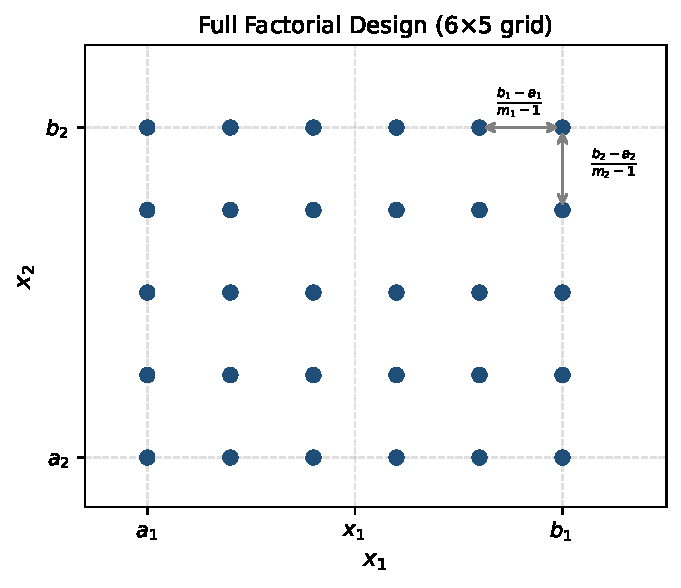
\includegraphics[width=\linewidth]{full_factorial}
    \vspace{0.2em}
    \small Grid of $6 \times 5 = 30$ points in 2D.
    Spacing labelled as $\frac{b_1-a_1}{m_1-1}$ and $\frac{b_2-a_2}{m_2-1}$.
  \end{columns}
\end{frame}

\begin{frame}[fragile]{Full Factorial --- Python Implementation}
  \begin{block}{Algorithm 16.1 (Python equivalent)}
    Return all grid locations for a full factorial plan.
    \texttt{a}, \texttt{b}: lower/upper bound vectors; \texttt{m}: sample counts per dimension.
  \end{block}
  \begin{lstlisting}[style=python, caption={Full factorial sampling (NumPy)}]
import numpy as np
from itertools import product

def samples_full_factorial(a, b, m):
    """
    a : array of lower bounds (length n)
    b : array of upper bounds (length n)
    m : array of sample counts per dimension (length n)
    Returns list of all grid points as numpy arrays.
    """
    grids = [np.linspace(a[i], b[i], m[i]) for i in range(len(a))]
    return [np.array(pt) for pt in product(*grids)]

# Example: 2D, 3x3 grid on [0,1]^2
pts = samples_full_factorial([0, 0], [1, 1], [3, 3])
print(f"Total points: {len(pts)}")   # 9
print("Points:", np.round(pts, 3))
  \end{lstlisting}
  \begin{columns}
    \column{0.5\textwidth}
    \begin{exampleblock}{Numerical Example}
      $n=2$, $m=[3,3]$, $a=[0,0]$, $b=[1,1]$:\\
      $\Delta_1 = \Delta_2 = 0.5$\\
      Points: $(0,0),(0,0.5),(0,1),\ldots,(1,1)$ --- \textbf{9 total}
    \end{exampleblock}
    \column{0.45\textwidth}
    \begin{exampleblock}{Complexity}
      Time: $\mathcal{O}(m^n)$\quad Space: $\mathcal{O}(m^n)$\\
      Practical only for $n \le 3$--$4$ dimensions.
    \end{exampleblock}
  \end{columns}
\end{frame}

% =============================================================================
\section{Random Sampling}
% =============================================================================

\begin{frame}[fragile]{16.2 Random Sampling}
  \begin{columns}
    \column{0.56\textwidth}
    \begin{block}{Method}
      Draw $m$ points independently from the design space.
      For bounded variable $x_i \in [a_i, b_i]$:
      \[
        x_i \sim \mathrm{Uniform}(a_i, b_i)
      \]
      Components are \emph{independent} across dimensions.
    \end{block}
    \begin{exampleblock}{Advantages}
      \begin{itemize}
        \item Trivially simple to implement
        \item No exponential blowup with $n$
        \item Unbiased --- no systematic structure
      \end{itemize}
    \end{exampleblock}
    \begin{alertblock}{Disadvantages}
      \begin{itemize}
        \item \textbf{Clustering}: points tend to clump by chance
        \item \textbf{Gaps}: large regions can be left uncovered
        \item Coverage quality degrades in high dimensions
      \end{itemize}
    \end{alertblock}

    \column{0.40\textwidth}
    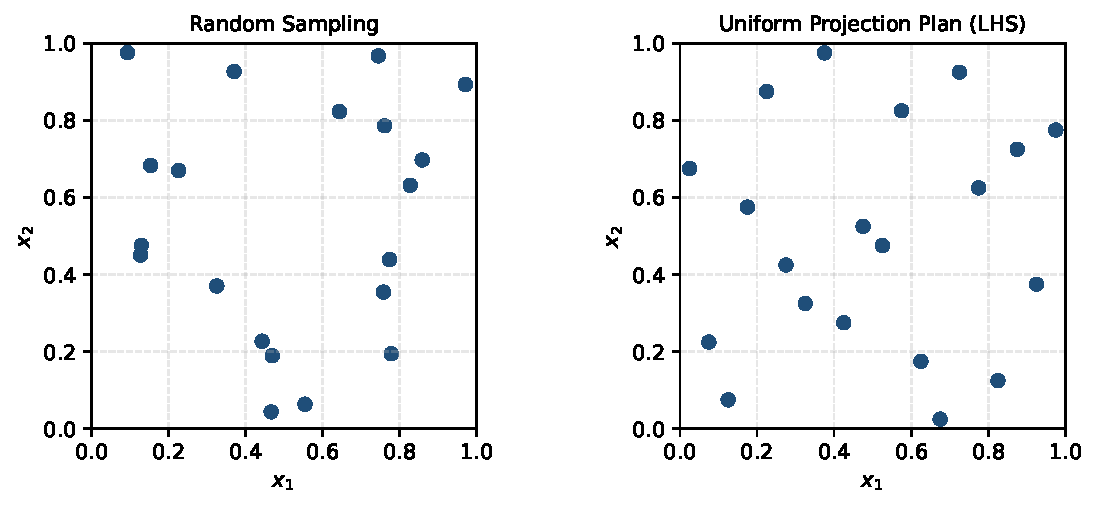
\includegraphics[width=\linewidth]{random_vs_projection}
    \vspace{0.3em}
    \small Left: random sampling (note clustering).\\
    Right: LHS --- uniform projection (better coverage).
  \end{columns}
\end{frame}

\begin{frame}[fragile]{Random Sampling --- Python}
  \begin{lstlisting}[style=python, caption={Random sampling with NumPy}]
import numpy as np

def random_sampling(a, b, m, seed=None):
    """
    Draw m random samples from the hypercube [a, b].
    a, b : lower/upper bound arrays (length n)
    m    : number of samples
    Returns (m x n) array.
    """
    rng = np.random.default_rng(seed)
    a, b = np.asarray(a, float), np.asarray(b, float)
    return a + rng.uniform(size=(m, len(a))) * (b - a)

# Example: 20 points in [0,1]^2
X = random_sampling([0, 0], [1, 1], 20, seed=42)
print(X.shape)   # (20, 2)

# Log-uniform sampling for step-size hyperparameters
def log_uniform_sampling(a, b, m, seed=None):
    rng = np.random.default_rng(seed)
    log_a, log_b = np.log(a), np.log(b)
    return np.exp(log_a + rng.uniform(size=(m, len(a))) * (log_b - log_a))
  \end{lstlisting}
  \vspace{0.3em}
  \begin{columns}
    \column{0.48\textwidth}
    \begin{exampleblock}{Note on Log-Uniform}
      Some parameters (e.g.\ neural network step size $\alpha$) are
      best searched in log-space:
      $\alpha \in [10^{-5}, 10^{-1}]$.
    \end{exampleblock}
    \column{0.46\textwidth}
    \begin{exampleblock}{Complexity}
      Time: $\mathcal{O}(mn)$\quad Space: $\mathcal{O}(mn)$\\
      Scales well but has no coverage guarantee.
    \end{exampleblock}
  \end{columns}
\end{frame}

% =============================================================================
\section{Uniform Projection Plans}
% =============================================================================

\begin{frame}{16.3 Uniform Projection Plans}
  \begin{columns}
    \column{0.55\textwidth}
    \begin{block}{Definition}
      A sampling plan $X$ over an $m \times m$ grid is a
      \textbf{uniform projection plan} if, when projected onto any
      single dimension, the $m$ samples are evenly distributed
      (one point per row, one per column --- like a Latin square).
    \end{block}
    \vspace{0.3em}
    \begin{block}{Latin Hypercube Sampling (LHS)}
      Generalization to $n$ dimensions:
      \begin{enumerate}
        \item Divide each dimension into $m$ equal strata of width $\frac{1}{m}$
        \item Assign exactly one sample to each stratum in each dimension
        \item Randomize within each stratum: $x_i^{(k)} \sim \mathrm{Uniform}\!\left(\frac{\sigma_k^{(i)}-1}{m},\,\frac{\sigma_k^{(i)}}{m}\right)$
      \end{enumerate}
      where $\boldsymbol{\sigma}^{(i)}$ is a random permutation of $\{1,\ldots,m\}$.
    \end{block}

    \column{0.41\textwidth}
    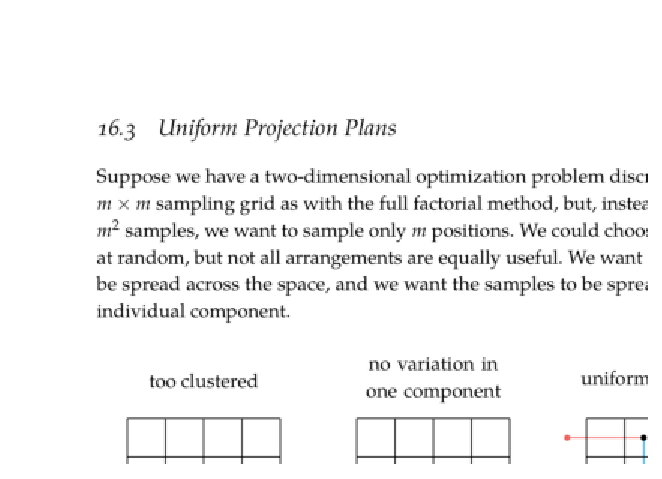
\includegraphics[width=\linewidth]{book_uniform_proj}
    \vspace{0.2em}
    \small Left: unconstrained random (3 in one column, none in another).\\
    Right: uniform projection (one per column).
  \end{columns}
\end{frame}

\begin{frame}[fragile]{Uniform Projection Plans --- Python}
  \begin{lstlisting}[style=python, caption={Latin Hypercube Sampling (Python/NumPy)}]
import numpy as np

def latin_hypercube_sample(m, n, seed=None):
    """
    Generate m-point Latin Hypercube Sampling in n dimensions, unit hypercube.
    m : number of samples
    n : number of dimensions
    Returns (m x n) array with values in [0, 1].
    """
    rng = np.random.default_rng(seed)
    X = np.zeros((m, n))
    for i in range(n):
        perm = rng.permutation(m)          # random permutation of strata
        offsets = rng.uniform(size=m)      # uniform within each stratum
        X[:, i] = (perm + offsets) / m
    return X

# Scale to [a, b]
def lhc_sample(a, b, m, seed=None):
    a, b = np.asarray(a, float), np.asarray(b, float)
    X01 = latin_hypercube_sample(m, len(a), seed)
    return a + X01 * (b - a)

# Example
X = lhc_sample([0, 0], [1, 1], 10, seed=7)
print("LHS plan (10 pts, 2D):\n", np.round(X, 3))

# Verify projection property: each stratum contains exactly 1 point
bins = (X * 10).astype(int)
print("x1 stratum counts:", np.bincount(bins[:,0]))  # all 1s
  \end{lstlisting}
\end{frame}

\begin{frame}{Uniform Projection Plans --- Properties}
  \begin{columns}
    \column{0.5\textwidth}
    \begin{block}{Key Property}
      For any one-dimensional projection onto dimension $i$,
      the $m$ points each fall in a distinct stratum
      $\left[\frac{k-1}{m},\,\frac{k}{m}\right]$ for $k=1,\ldots,m$.
    \end{block}
    \vspace{0.3em}
    \begin{exampleblock}{Numerical Example ($m=5$, $n=2$)}
      Strata in $x_1$: $[0,0.2), [0.2,0.4), [0.4,0.6), [0.6,0.8), [0.8,1]$\\
      Each stratum gets \emph{exactly one} point.\\
      Same guarantee for $x_2$.
    \end{exampleblock}
    \begin{alertblock}{Limitation}
      Uniform projection is guaranteed only for 1D marginals.
      Pairs of dimensions may still cluster (in higher $n$).
    \end{alertblock}

    \column{0.46\textwidth}
    \begin{block}{Algorithm 16.2 (Python)}
      \texttt{sample\_uniform\_projection(m)} generates an $m$-point
      uniform projection plan over $\{1,\ldots,m\}^n$:
      \begin{enumerate}
        \item For each dimension $i$: draw random permutation $\sigma^{(i)}$ of $1\ldots m$
        \item Return $\{(\sigma^{(1)}_k, \sigma^{(2)}_k, \ldots, \sigma^{(n)}_k)\}_{k=1}^m$
      \end{enumerate}
    \end{block}
    \vspace{0.3em}
    Total possible plans in 2D: $m!$ (only $m$ of $m^m$ grids are valid UPPs).\\
    For $m=10$: $10! = 3{,}628{,}800$ possible plans.
  \end{columns}
\end{frame}

% =============================================================================
\section{Stratified Sampling}
% =============================================================================

\begin{frame}[fragile]{16.4 Stratified Sampling}
  \begin{columns}
    \column{0.52\textwidth}
    \begin{block}{Concept}
      Divide the design space into non-overlapping \textbf{strata} (sub-regions).
      Draw at least one sample from each stratum.
      \[
        X = X_1 \cup X_2 \cup \cdots \cup X_k,
        \quad X_i \cap X_j = \emptyset
      \]
      This prevents large empty regions from occurring.
    \end{block}
    \vspace{0.3em}
    \begin{block}{Relation to Projection Plans}
      Stratified sampling $\supseteq$ LHS:
      \begin{itemize}
        \item \textbf{Pure stratified}: one point per 2D cell (factorial structure, $m^2$ total)
        \item \textbf{LHS / UPP}: one point per row \emph{and} per column, $m$ total
        \item LHS is a more efficient form of stratified sampling
      \end{itemize}
    \end{block}

    \column{0.44\textwidth}
    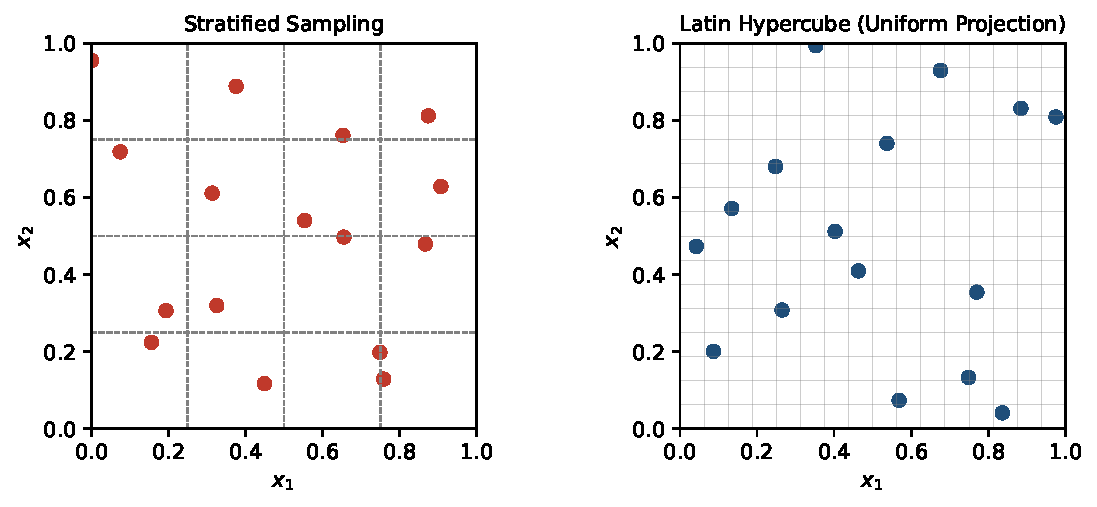
\includegraphics[width=\linewidth]{stratified_sampling}
    \vspace{0.2em}
    \small Left: grid-stratified (one point per 2D cell).\\
    Right: Latin Hypercube (one per row \& column stratum).
  \end{columns}
\end{frame}

\begin{frame}[fragile]{Stratified Sampling --- Python}
  \begin{lstlisting}[style=python, caption={Stratified sampling in Python}]
import numpy as np

def stratified_sample(a, b, m_per_dim, seed=None):
    """
    Grid-stratified sampling: one random point per cell.
    a, b        : bound vectors (length n)
    m_per_dim   : number of strata per dimension (list of ints)
    Returns array of shape (prod(m_per_dim), n).
    """
    from itertools import product
    rng = np.random.default_rng(seed)
    a, b = np.asarray(a, float), np.asarray(b, float)
    n = len(a)
    # stratum edges for each dimension
    edges = [np.linspace(a[i], b[i], m_per_dim[i] + 1) for i in range(n)]
    pts = []
    for idx in product(*[range(m) for m in m_per_dim]):
        pt = [rng.uniform(edges[i][idx[i]], edges[i][idx[i]+1])
              for i in range(n)]
        pts.append(pt)
    return np.array(pts)

# Example: 3x3 strata in 2D
X = stratified_sample([0,0], [1,1], [3,3], seed=0)
print(f"Points: {len(X)}")  # 9
  \end{lstlisting}
  \vspace{0.2em}
  \begin{exampleblock}{Key difference from LHS}
    Grid-stratified: $\prod m_i$ total points (quadratic in 2D).
    LHS: $m$ points, $m$ strata per dimension --- much more efficient!
  \end{exampleblock}
\end{frame}

% =============================================================================
\section{Space-Filling Metrics}
% =============================================================================

\begin{frame}{16.5 Space-Filling Metrics --- Overview}
  \begin{columns}
    \column{0.55\textwidth}
    To \emph{compare} sampling plans, we need a quantitative metric.
    Two key families:
    \begin{enumerate}
      \item \textbf{Discrepancy} --- how much does the empirical distribution
            deviate from uniform?
      \item \textbf{Fill Distance} --- what is the largest uncovered region?
    \end{enumerate}
    \vspace{0.5em}
    Both measure different aspects of ``how well does $X$ cover $\mathcal{X}$?''
    \begin{block}{Setup}
      Design space: $\mathcal{X} = [0,1]^n$ (unit hypercube)\\
      Sampling plan: $X = \{\mathbf{x}^{(1)},\ldots,\mathbf{x}^{(m)}\}$
    \end{block}

    \column{0.41\textwidth}
    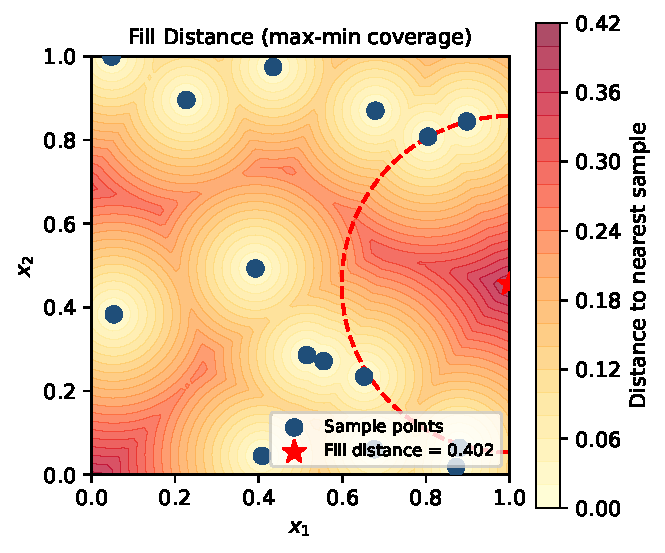
\includegraphics[width=\linewidth]{fill_distance}
    \vspace{0.2em}
    \small Heatmap of distance-to-nearest-sample.
    Fill distance = radius of largest empty circle (red star).
  \end{columns}
\end{frame}

\begin{frame}{16.5.1 Discrepancy}
  \begin{columns}
    \column{0.54\textwidth}
    \begin{block}{Definition (Star Discrepancy)}
      For a set $X$ of $m$ points and a rectangular subset $H \subseteq [0,1]^n$:
      \[
        D(X) = \sup_{H \subseteq [0,1]^n}
          \left|\frac{\#(X \cap H)}{m} - \mathrm{Vol}(H)\right|
      \]
      where the supremum is over all axis-aligned rectangles $H$.
    \end{block}
    \begin{block}{Interpretation}
      \begin{itemize}
        \item $\frac{\#(X \cap H)}{m}$: fraction of points in $H$
        \item $\mathrm{Vol}(H)$: fraction of volume in $H$
        \item $D(X)$ = maximum mismatch between empirical and uniform
        \item \textbf{Low discrepancy} $\Rightarrow$ better coverage
      \end{itemize}
    \end{block}

    \column{0.42\textwidth}
    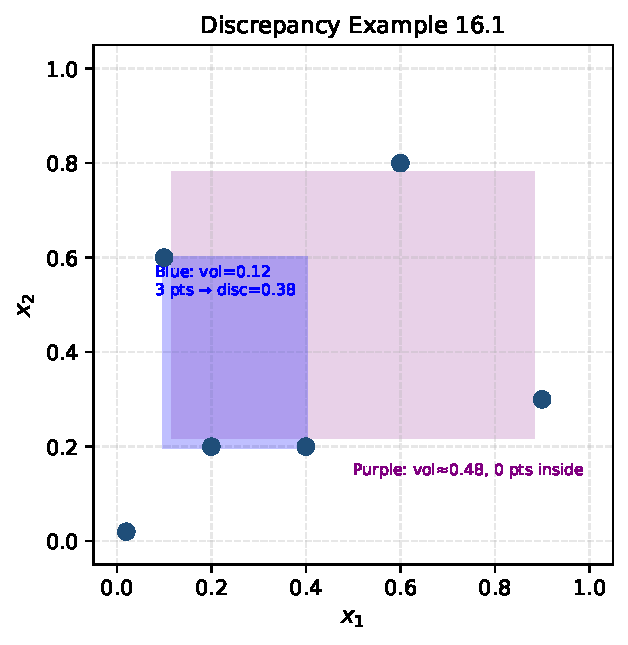
\includegraphics[width=\linewidth]{discrepancy_example}
    \vspace{0.2em}
    \small\textbf{Example 16.1:}
    Blue rectangle: $x_1\in[\tfrac{1}{10},\tfrac{2}{5}]$,
    $x_2\in[\tfrac{1}{5},\tfrac{3}{5}]$,
    Vol $= 0.12$, contains 3 pts.\\
    Discrepancy: $\left|\tfrac{3}{6} - 0.12\right| = 0.38$
  \end{columns}
\end{frame}

\begin{frame}[allowframebreaks]{16.5.1 Discrepancy --- Worked Example}
  \begin{exampleblock}{Example 16.1 from the book}
    Consider the 6-point set:
    \[
      X = \left\{
        \begin{bmatrix}1/5\\1/5\end{bmatrix},
        \begin{bmatrix}2/5\\1/5\end{bmatrix},
        \begin{bmatrix}1/10\\3/5\end{bmatrix},
        \begin{bmatrix}9/10\\3/10\end{bmatrix},
        \begin{bmatrix}1/50\\1/50\end{bmatrix},
        \begin{bmatrix}3/5\\4/5\end{bmatrix}
      \right\}
    \]
    \textbf{Blue rectangle}: $x_1 \in [1/10, 2/5]$, $x_2 \in [1/5, 3/5]$
    \begin{itemize}
      \item Volume $= (2/5-1/10)\times(3/5-1/5) = 0.3\times 0.4 = 0.12$
      \item Contains points: $(1/5,1/5)$, $(2/5,1/5)$, $(1/10,3/5)$ --- \textbf{3 points}
      \item Discrepancy measure: $|3/6 - 0.12| = |0.5 - 0.12| = \mathbf{0.38}$
    \end{itemize}

    \textbf{Purple rectangle}: $x_1 \in [1/10+\epsilon, 9/10-\epsilon]$,
    $x_2 \in [1/5+\epsilon, 4/5-\epsilon]$
    \begin{itemize}
      \item As $\epsilon \to 0$: Volume $\to (0.8)\times(0.6) = 0.48$
      \item Contains \textbf{0 points} (just misses all of them)
      \item Discrepancy: $|0/6 - 0.48| = \mathbf{0.48}$ (even worse!)
    \end{itemize}

    The \textbf{supremum} (over all rectangles) gives $D(X) = 0.48$.
    Note: we need the \emph{supremum} because the maximum is approached
    in the limit $\epsilon \to 0$.
  \end{exampleblock}

  \framebreak

  \begin{columns}
    \column{0.52\textwidth}
    \begin{block}{Properties of Discrepancy}
      \begin{itemize}
        \item $D(X) \in [0, 1]$
        \item $D(X) = 0$ only for perfectly uniform distribution
        \item For $m$ uniform random points:
              $D(X) = \mathcal{O}((\log m)^n / m)$ in expectation
        \item Low-discrepancy sequences achieve
              $D(X) = \mathcal{O}((\log m)^n / m)$ \emph{deterministically}
      \end{itemize}
    \end{block}
    \begin{alertblock}{Computational Complexity}
      Exact discrepancy is NP-hard to compute for $n > 1$.
      Computing $D(X)$ efficiently requires special algorithms.
    \end{alertblock}

    \column{0.44\textwidth}
    \begin{block}{Alternative: $L_2$ Discrepancy}
      Replace sup with $L_2$ norm (easier to compute):
      \[
        D_2(X) = \left[\int_{[0,1]^n}
          \left|\frac{\#(X\cap H_\mathbf{t})}{m} - \mathrm{Vol}(H_\mathbf{t})\right|^2
          d\mathbf{t}\right]^{1/2}
      \]
      where $H_\mathbf{t} = [0,t_1]\times\cdots\times[0,t_n]$.
    \end{block}
  \end{columns}
\end{frame}

\begin{frame}{16.5.2 Fill Distance (Packing Distance)}
  \begin{columns}
    \column{0.52\textwidth}
    \begin{block}{Fill Distance}
      The \textbf{fill distance} (covering radius) measures the
      worst-case distance from any point in $\mathcal{X}$ to its
      nearest sample:
      \[
        d_{\mathrm{fill}}(X, \mathcal{X}) =
          \sup_{\mathbf{z} \in \mathcal{X}}\;
          \min_{\mathbf{x} \in X}\;
          \|\mathbf{z} - \mathbf{x}\|_p
      \]
    \end{block}
    \begin{block}{Pairwise Distances (Algorithm 16.3)}
      To assess coverage, compute all pairwise $L_p$ distances:
      \[
        D_{\mathrm{pairs}}(X,p) = \bigl\{\|\mathbf{x}^{(i)} - \mathbf{x}^{(j)}\|_p
          \;\big|\; i < j\bigr\}
      \]
      Minimum pairwise distance = \emph{packing distance}.\\
      Want: large min distance AND small fill distance.
    \end{block}

    \column{0.44\textwidth}
    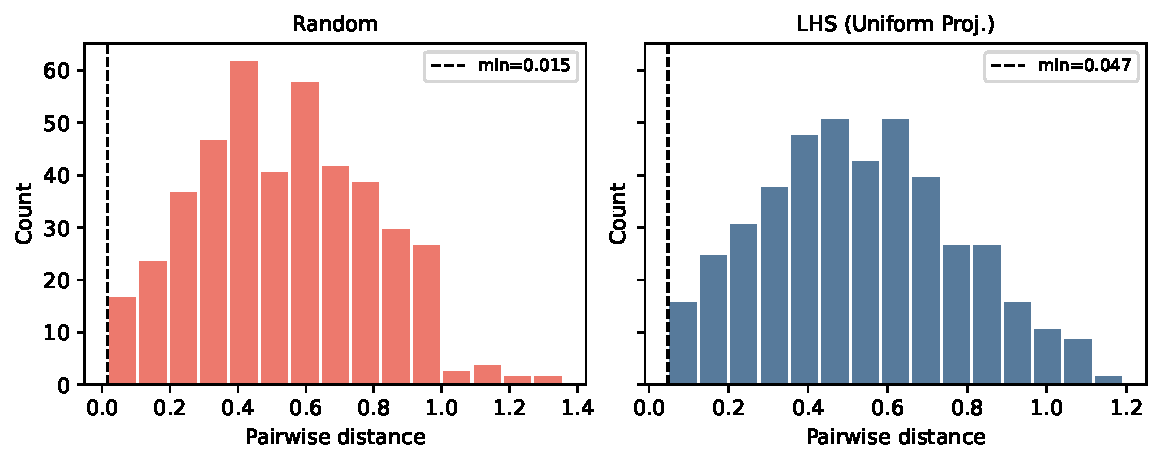
\includegraphics[width=\linewidth]{pairwise_distances}
    \vspace{0.2em}
    \small Pairwise distance histograms for 30-point plans.
    LHS (right) has larger minimum pairwise distances.
  \end{columns}
\end{frame}

\begin{frame}[fragile]{Pairwise Distances --- Python}
  \begin{lstlisting}[style=python, caption={Algorithm 16.3 in Python}]
import numpy as np
from scipy.spatial.distance import pdist

def pairwise_distances(X, p=2):
    """
    X : (m x n) array of sample points
    p : L_p norm (default: Euclidean p=2)
    Returns array of all m*(m-1)/2 pairwise distances.
    """
    # Direct loop (as in book)
    m = len(X)
    dists = [np.linalg.norm(X[i] - X[j], ord=p)
             for i in range(m-1) for j in range(i+1, m)]
    return np.array(dists)

# Using scipy (faster):
def pairwise_distances_scipy(X, p=2):
    return pdist(X, metric='minkowski', p=p)

# Compare two plans
X_rand = np.random.default_rng(0).uniform(0, 1, (20, 2))
X_lhc  = latin_hypercube_sample(20, 2, seed=0)  # from earlier

dr = pairwise_distances(X_rand)
dl = pairwise_distances(X_lhc)
print(f"Random: min dist = {dr.min():.4f}")
print(f"LHS:    min dist = {dl.min():.4f}")  # typically larger
  \end{lstlisting}
\end{frame}

% =============================================================================
\section{Space-Filling Subsets (MaxMin / MaxDet)}
% =============================================================================

\begin{frame}{16.5.3 Morris-Mitchell Criterion}
  \begin{columns}
    \column{0.54\textwidth}
    \begin{block}{Morris-Mitchell $\Phi_q$ Criterion (Eq.\ 16.2)}
      For a sampling plan $X$ with pairwise distances $\{d_i\}$:
      \[
        \Phi_q(X) = \left(\sum_i d_i^{-q}\right)^{1/q}
      \]
      where $q > 0$ is a tunable parameter.
      \begin{itemize}
        \item $q$ large: emphasizes the \emph{smallest} distance
        \item $q=1$: harmonic mean-like; spread over all distances
        \item We want to \textbf{minimize} $\Phi_q$
      \end{itemize}
    \end{block}
    \begin{block}{Optimization Problem (Eq.\ 16.3)}
      \[
        \underset{X}{\text{minimize}}\;
        \underset{\boldsymbol{\sigma}}{\text{maximize}}\;
        \Phi_q(X)
      \]
      over all UPPs $X$ (uniform projection plans).
    \end{block}

    \column{0.42\textwidth}
    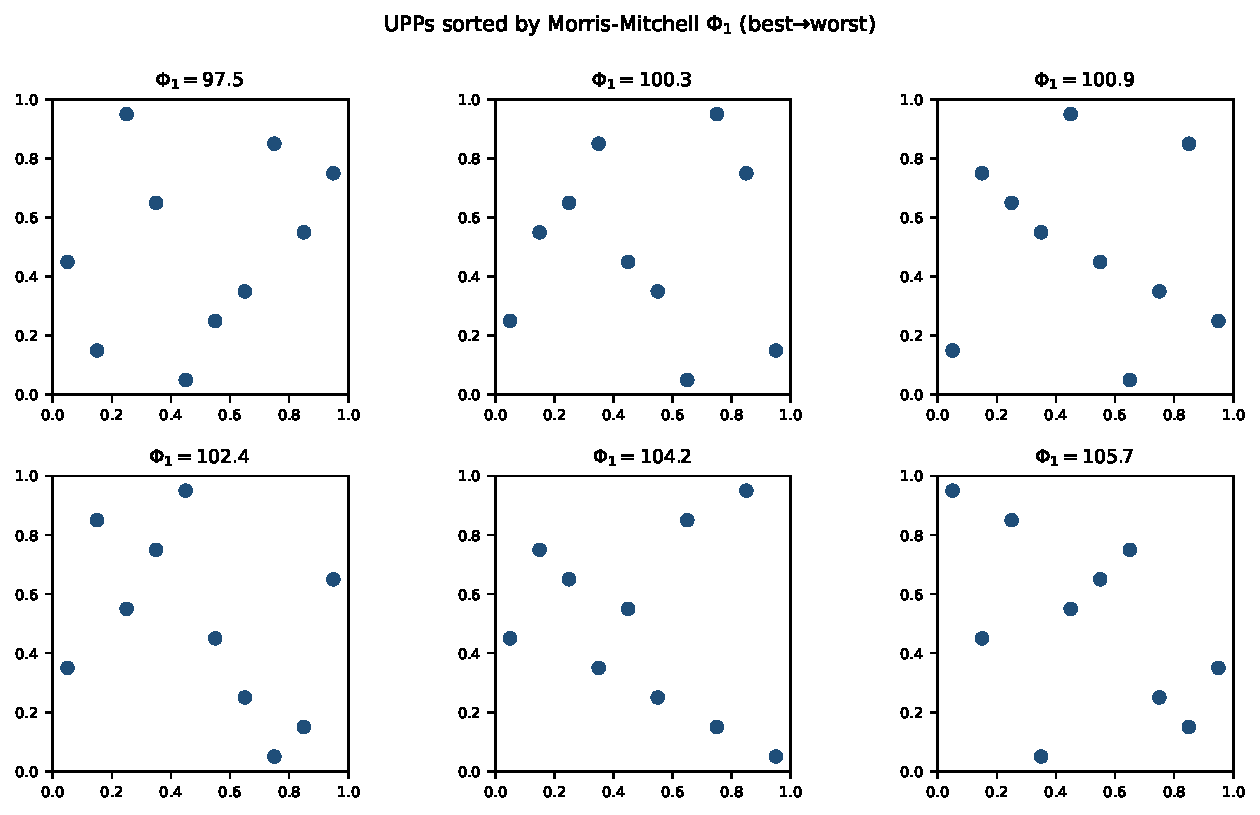
\includegraphics[width=\linewidth]{morris_mitchell}
    \vspace{0.2em}
    \small Six random LHS plans sorted by $\Phi_1$.
    Lower $\Phi_1$ = better space-filling.
  \end{columns}
\end{frame}

\begin{frame}[fragile]{Morris-Mitchell --- Python + Mutation Algorithm}
  \begin{lstlisting}[style=python, caption={Morris-Mitchell criterion + random mutation}]
import numpy as np

def phi_q(X, q=1):
    """Morris-Mitchell criterion. Minimize this."""
    dists = pdist(X)          # all pairwise L2 distances
    return np.sum(dists**(-q))**(1/q)

def compare_sampling_plans(A, B, p=2, q=1):
    """Return 1 if A is more space-filling than B, -1 if B, 0 if equal."""
    da = np.sort(pdist(A, metric='minkowski', p=p))
    db = np.sort(pdist(B, metric='minkowski', p=p))
    for a, b in zip(da, db):
        if a < b: return -1   # A has smaller min distance => B better
        if a > b: return  1
    return 0

def mutate(X):
    """Swap two values in a random column (Algorithm 16.5 in book).
    Maintains uniform projection property."""
    X2 = X.copy()
    m, n = X2.shape
    col = np.random.randint(n)
    i, j = np.random.choice(m, 2, replace=False)
    X2[i, col], X2[j, col] = X2[j, col], X2[i, col]
    return X2

# Stochastic optimization of LHS
def optimize_lhs(m, n, n_iter=2000, q=1, seed=42):
    rng = np.random.default_rng(seed)
    X = latin_hypercube_sample(m, n, seed=seed)
    best_phi = phi_q(X, q)
    for _ in range(n_iter):
        X2 = mutate(X)
        phi2 = phi_q(X2, q)
        if phi2 < best_phi:
            X, best_phi = X2, phi2
    return X, best_phi
  \end{lstlisting}
\end{frame}

% =============================================================================
\section{Space-Filling Subsets}
% =============================================================================

\begin{frame}{16.6 Space-Filling Subsets}
  \begin{columns}
    \column{0.55\textwidth}
    \begin{block}{Problem}
      Given a large set $X$ of design points, find a \emph{subset}
      $S \subset X$, $|S| = m$, that still ``maximally fills'' $X$.
      \[
        d(A, B) = \max_{\mathbf{x} \in A}\; \min_{\mathbf{y} \in B}\;
          \|\mathbf{x} - \mathbf{y}\|_p
      \]
      Minimize the fill distance: $\min_S\; d(X, S)$.
    \end{block}
    \begin{block}{Application}
      Multifidelity models: use $X$ (cheap simulation) to identify
      $m$ design points to evaluate with expensive high-fidelity model.
      E.g., wind-tunnel testing of aircraft wing designs.
    \end{block}
    \begin{alertblock}{Optimization}
      Exact minimization is NP-hard.
      Two practical approaches:
      (1) Greedy selection (Alg.\ 16.8),
      (2) Exchange selection (Alg.\ 16.9).
    \end{alertblock}

    \column{0.41\textwidth}
    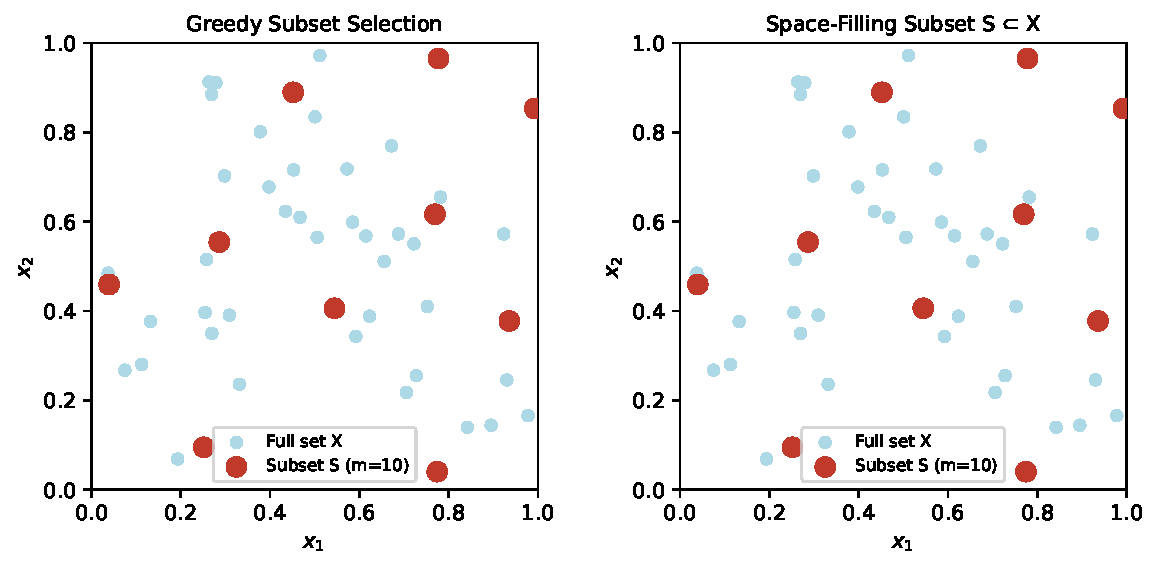
\includegraphics[width=\linewidth]{subset_selection}
    \vspace{0.2em}
    \small Blue dots: full candidate set $X$.
    Red dots: space-filling subset $S \subset X$ (greedy selection, $m=10$).
  \end{columns}
\end{frame}

\begin{frame}[fragile]{16.6 Greedy Subset Selection (Algorithm 16.8)}
  \begin{lstlisting}[style=python, caption={Greedy space-filling subset selection}]
import numpy as np
from scipy.spatial.distance import cdist

def greedy_subset_selection(X, m, p=2):
    """
    Algorithm 16.8: Greedy subset selection.
    Builds an m-point subset that minimizes fill distance d(X, S).
    X : (N x n) array --- full candidate set
    m : desired subset size
    p : L_p norm
    Returns list of indices into X.
    """
    N = len(X)
    rng = np.random.default_rng(0)
    S = [rng.integers(N)]           # start with one random point

    for _ in range(m - 1):
        # For each candidate NOT in S:
        # find its distance to the current subset S
        S_arr = X[S]
        # cdist: shape (N, |S|)
        dists = cdist(X, S_arr, metric='minkowski', p=p)
        # distance from each x to nearest point in S
        d_to_S = dists.min(axis=1)
        # mask out already-selected points
        d_to_S[S] = -np.inf
        # pick the point FARTHEST from S  (minimizes fill distance)
        best = int(np.argmax(d_to_S))
        S.append(best)

    return S

# Example
X = np.random.default_rng(1).uniform(0,1,(100,2))
idx = greedy_subset_selection(X, 10)
S = X[idx]
  \end{lstlisting}
\end{frame}

\begin{frame}[fragile]{16.6 Exchange Subset Selection (Algorithm 16.9)}
  \begin{lstlisting}[style=python, caption={Exchange subset selection (local search)}]
def exchange_subset_selection(X, m, p=2):
    """
    Algorithm 16.9: Exchange-based subset selection.
    Iteratively swaps elements of S with points in X \ S
    to reduce fill distance.
    """
    from scipy.spatial.distance import cdist
    rng = np.random.default_rng(0)
    S_idx = list(rng.choice(len(X), m, replace=False))

    def fill_dist(S_idx):
        S = X[S_idx]
        dists = cdist(X, S).min(axis=1)
        return dists.max()

    delta = fill_dist(S_idx)
    done = False
    while not done:
        best_pair = None
        for i in range(m):
            old = S_idx[i]
            for j, x in enumerate(X):
                if j in S_idx:
                    continue
                S_idx[i] = j
                delta_prime = fill_dist(S_idx)
                if delta_prime < delta:
                    delta = delta_prime
                    best_pair = (i, j)
                S_idx[i] = old
        done = (best_pair is None)
        if not done:
            i, j = best_pair
            S_idx[i] = j   # commit the best swap
    return S_idx
  \end{lstlisting}
  \begin{exampleblock}{Complexity}
    Each iteration: $\mathcal{O}(m \cdot N)$ distance evaluations.
    Converges to local optimum; typically much better than greedy alone.
  \end{exampleblock}
\end{frame}

% =============================================================================
\section{Quasi-Random Sequences}
% =============================================================================

\begin{frame}{16.7 Quasi-Random Sequences}
  \begin{columns}
    \column{0.55\textwidth}
    \begin{block}{Definition}
      \textbf{Quasi-random sequences} (low-discrepancy sequences) are
      \emph{deterministic} sequences that fill the unit hypercube more
      uniformly than pseudo-random sequences.

      \vspace{0.3em}
      Key property: when $\mathbf{x}^{(k)}$ is sampled, the error in
      Monte Carlo integration satisfies:
      \[
        \left|\frac{1}{m}\sum_{k=1}^m f(\mathbf{x}^{(k)}) - \int f\right|
          = \mathcal{O}\!\left(\frac{(\log m)^n}{m}\right)
      \]
      versus $\mathcal{O}(m^{-1/2})$ for random sampling.
    \end{block}
    \begin{alertblock}{Note}
      These sequences are \emph{not} random.
      They are called ``quasi-random'' to emphasize their
      random-like coverage properties while being deterministic.
    \end{alertblock}

    \column{0.41\textwidth}
    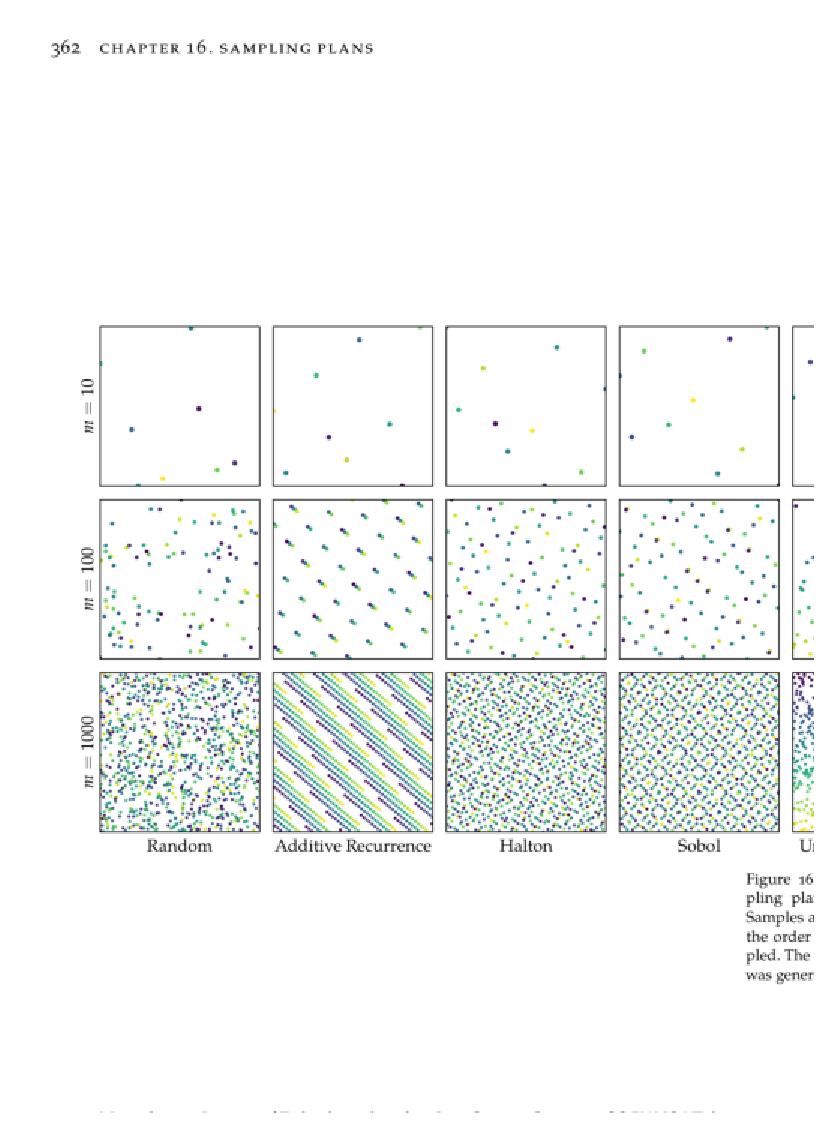
\includegraphics[width=\linewidth]{book_comparison}
    \vspace{0.2em}
    \small Figure 16.13: All five methods at $n=10, 100, 1000$.
    Quasi-random methods (Halton, Sobol) show more uniform coverage.
  \end{columns}
\end{frame}

\begin{frame}{16.7.1 Additive Recurrence}
  \begin{columns}
    \column{0.54\textwidth}
    \begin{block}{Method (Eq.\ 16.7)}
      Generate a sequence in $[0,1]$ using:
      \[
        x^{(k+1)} = \bigl(x^{(k)} + c\bigr) \bmod 1
      \]
      where $c$ is \textbf{irrational}.
      Explicit form: $x^{(k)} = (x^{(0)} + kc) \bmod 1$.
    \end{block}
    \begin{block}{Choice of $c$}
      \begin{itemize}
        \item Best 1D: $c = \phi - 1 = \frac{\sqrt{5}-1}{2} \approx 0.618$
              (golden ratio conjugate)
        \item For $n$ dimensions: use $c_i = \sqrt{p_i}$ where
              $p_i$ is the $i$-th prime
        \item \textbf{Must be irrational}: rational $c = a/b$ gives
              period $b$ (sequence repeats!)
      \end{itemize}
    \end{block}
    \begin{alertblock}{Exercise 16.4}
      If $c = a/b$ (rational), then $x^{(k+b)} = x^{(k)}$ for all $k$.
      The sequence repeats with period $b$ --- not space-filling!
    \end{alertblock}

    \column{0.42\textwidth}
    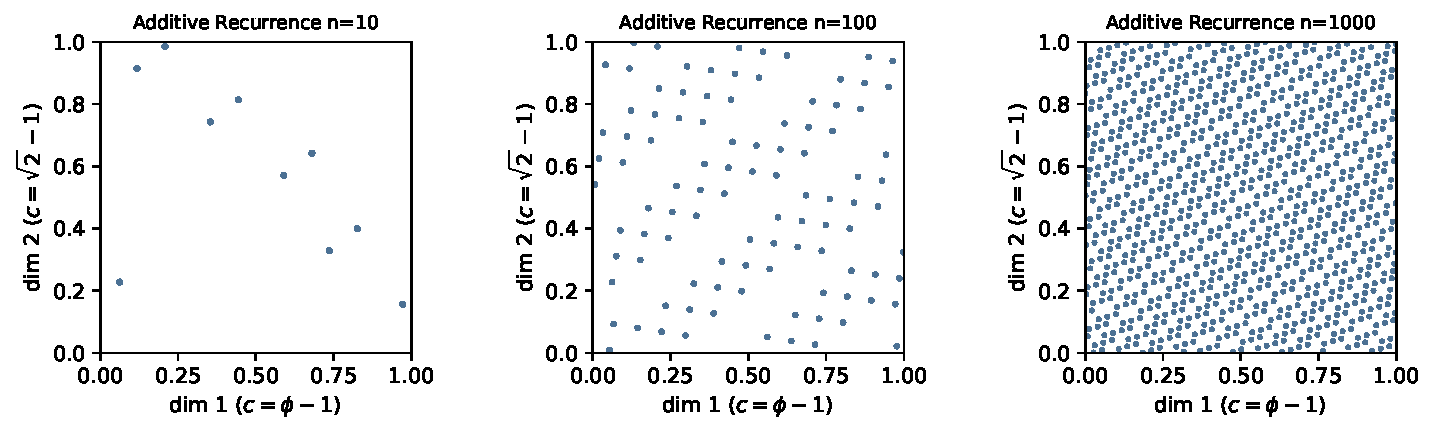
\includegraphics[width=\linewidth]{additive_recurrence}
    \vspace{0.2em}
    \small Additive recurrence at $n=10, 100, 1000$ samples.
    Diagonal stripes are visible --- correlation between dimensions.
  \end{columns}
\end{frame}

\begin{frame}[fragile]{Additive Recurrence --- Python (Algorithm 16.10)}
  \begin{lstlisting}[style=python, caption={Additive recurrence sequences}]
import numpy as np

def filling_set_additive_recurrence(m, c=None):
    """
    1D additive recurrence sequence.
    m : number of points
    c : step size (default: golden ratio conjugate phi-1)
    """
    if c is None:
        phi = (1 + np.sqrt(5)) / 2
        c = phi - 1   # ~0.6180339887...
    x0 = np.random.rand()
    return np.array([(x0 + k * c) % 1.0 for k in range(1, m + 1)])

def filling_set_additive_recurrence_nd(m, n):
    """
    n-dimensional additive recurrence.
    Uses c_i = sqrt(prime_i) for dimension i.
    """
    def nth_prime(k):
        """Return the k-th prime (1-indexed)."""
        primes, x = [], 2
        while len(primes) < k:
            if all(x % p != 0 for p in primes):
                primes.append(x)
            x += 1
        return primes[k-1]

    seqs = [filling_set_additive_recurrence(m, c=np.sqrt(nth_prime(i+1)))
            for i in range(n)]
    return np.column_stack(seqs)

# Example: 100 points in 2D
X = filling_set_additive_recurrence_nd(100, 2)
print(X.shape)   # (100, 2)
  \end{lstlisting}
\end{frame}

\begin{frame}{16.7.2 Halton Sequence}
  \begin{columns}
    \column{0.55\textwidth}
    \begin{block}{Van der Corput Construction}
      For base $b$, the $i$-th Halton value is obtained by
      \emph{reflecting} the base-$b$ representation of $i$ around
      the decimal point:
      \[
        i = \sum_{k=0}^{\infty} a_k(i)\, b^k
        \quad\Rightarrow\quad
        \mathrm{halton}(i, b) = \sum_{k=0}^{\infty} a_k(i)\, b^{-(k+1)}
      \]
    \end{block}
    \begin{block}{Examples (Eqs.\ 16.10--16.11)}
      Base $b=2$:
      \[
        X = \left\{\frac{1}{2},\frac{1}{4},\frac{3}{4},\frac{1}{8},\frac{3}{8},
                    \frac{5}{8},\frac{7}{8},\frac{1}{16},\ldots\right\}
      \]
      Base $b=5$:
      \[
        X = \left\{\frac{1}{5},\frac{2}{5},\frac{3}{5},\frac{4}{5},
                    \frac{1}{25},\frac{6}{25},\frac{11}{25},\ldots\right\}
      \]
    \end{block}

    \column{0.41\textwidth}
    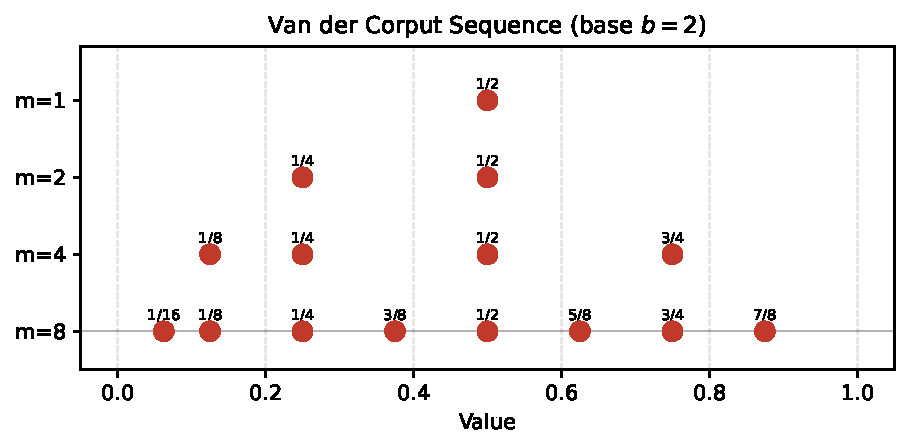
\includegraphics[width=\linewidth]{halton_tree}
    \vspace{0.2em}
    \small Van der Corput sequence (base 2) progressively fills $[0,1]$.
    Each new point fills the largest gap.

    \vspace{0.4em}
    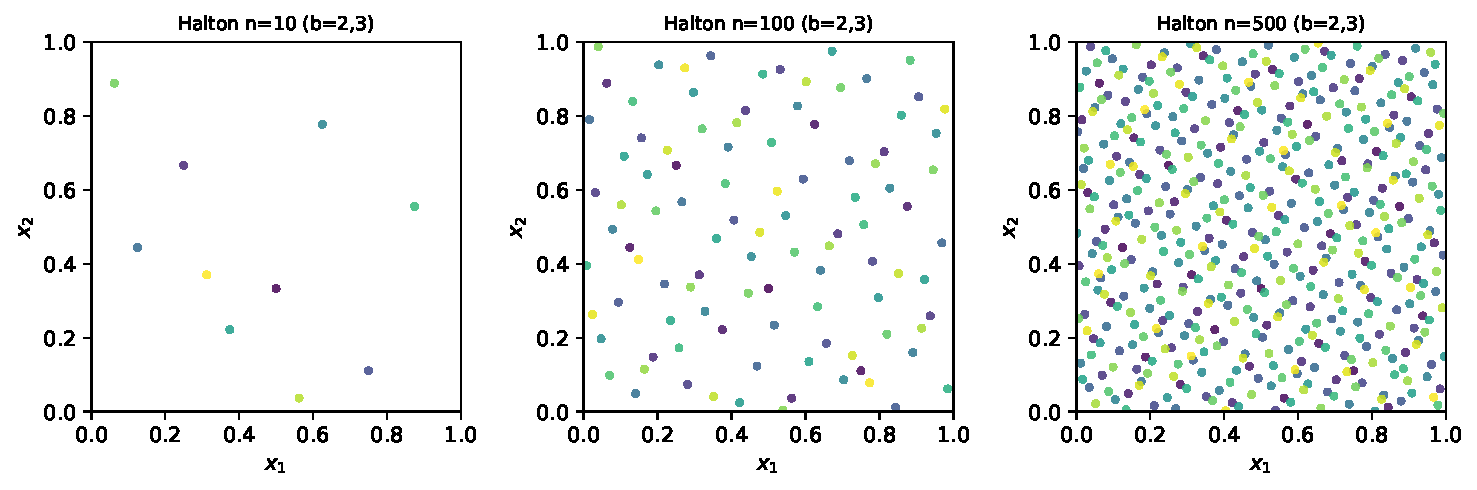
\includegraphics[width=\linewidth]{halton_2d}
    \vspace{0.1em}
    \small 2D Halton (bases 2 and 3) at $n=10, 100, 500$.
  \end{columns}
\end{frame}

\begin{frame}[fragile]{Halton Sequence --- Python (Algorithm 16.11)}
  \begin{lstlisting}[style=python, caption={Halton and van der Corput sequence}]
import numpy as np

def halton(i, b):
    """
    i-th element of the van der Corput sequence in base b.
    i : 1-indexed integer
    b : base (must be prime for coprimality)
    """
    result, f = 0.0, 1.0
    while i > 0:
        f /= b
        result += f * (i % b)
        i = i // b
    return result

def filling_set_halton(m, b=2):
    """1D Halton sequence of length m in base b."""
    return np.array([halton(i, b) for i in range(1, m + 1)])

def filling_set_halton_nd(m, n):
    """n-dimensional Halton sequence using first n prime bases."""
    from sympy import prime   # or use a precomputed list
    primes = [2, 3, 5, 7, 11, 13, 17, 19, 23, 29]  # first 10 primes
    assert n <= len(primes), f"Need at most {len(primes)} dimensions"
    seqs = [filling_set_halton(m, b=primes[i]) for i in range(n)]
    return np.column_stack(seqs)

# Numerical example: first 8 values, base 2
seq = filling_set_halton(8, b=2)
print(seq.round(4))
# [0.5, 0.25, 0.75, 0.125, 0.625, 0.375, 0.875, 0.0625]
  \end{lstlisting}
\end{frame}

\begin{frame}[fragile]{16.7.3 Sobol Sequence}
  \begin{columns}
    \column{0.55\textwidth}
    \begin{block}{Sobol Sequences}
      Sobol sequences are $n$-dimensional quasi-random sequences
      based on \textbf{base-2} digit scrambling using direction numbers.
      \begin{itemize}
        \item Each dimension uses a different set of \emph{direction numbers}
              $v_1, v_2, \ldots$ (derived from primitive polynomials over $\mathbb{F}_2$)
        \item The $k$-th sample is:
              $x_i^{(k)} = k_1 v_1 \oplus k_2 v_2 \oplus \cdots$ (bitwise XOR)
        \item Sobol sequences are better than Halton for higher dimensions
              (Halton shows correlation for large prime bases)
      \end{itemize}
    \end{block}
    \begin{block}{Python: scipy.stats.qmc}
      SciPy provides a production-quality Sobol generator.
    \end{block}

    \column{0.41\textwidth}
    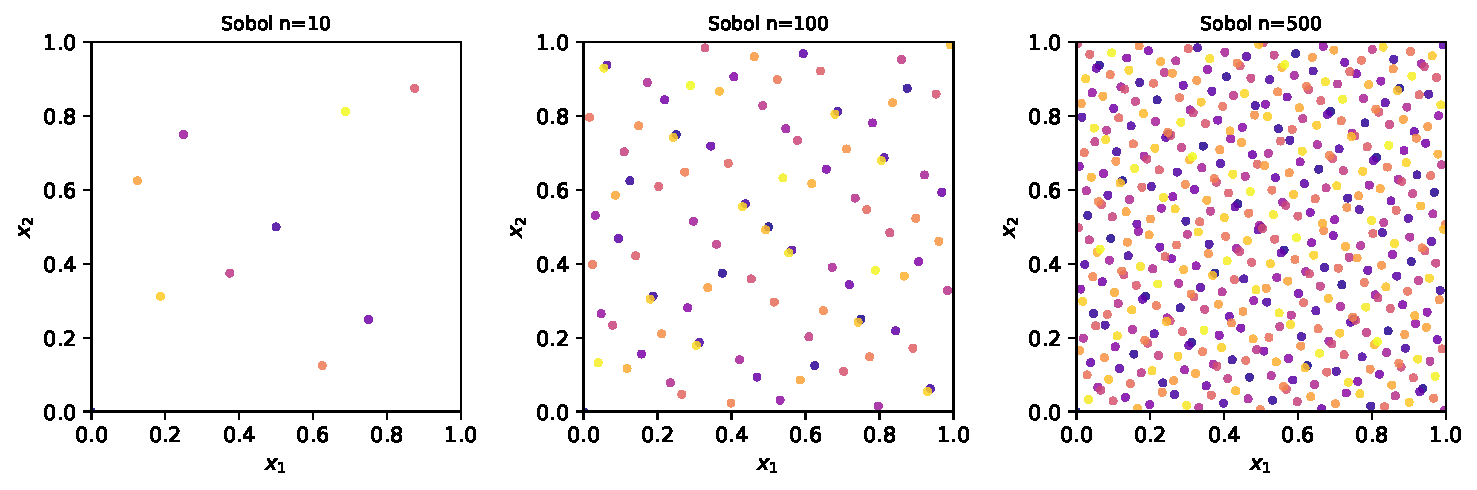
\includegraphics[width=\linewidth]{sobol_2d}
    \vspace{0.2em}
    \small Sobol sequence in 2D at $n=10, 100, 500$.
    Points fill space very uniformly (diagonal structure visible at small $n$).

    \vspace{0.3em}
    \begin{alertblock}{Important}
      Best results when $m$ is a power of 2
      (Sobol has exact equidistribution at $2^k$ points).
    \end{alertblock}
  \end{columns}
\end{frame}

\begin{frame}[fragile]{Sobol Sequence --- Python}
  \begin{lstlisting}[style=python, caption={Sobol sequence using scipy.stats.qmc}]
import numpy as np
from scipy.stats import qmc

# --- Sobol sequence -----------------------------------------------
def sobol_sample(m, n, scramble=True, seed=42):
    """
    Generate m Sobol points in n dimensions.
    scramble: use randomized (Owen) scrambling for better uniformity
    For best equidistribution, choose m = 2^k.
    """
    sampler = qmc.Sobol(d=n, scramble=scramble, seed=seed)
    X = sampler.random_base2(m=int(np.log2(m)))  # m must be power of 2
    return X

# Scale to [a, b]
def sobol_sample_scaled(a, b, m, scramble=True, seed=42):
    a, b = np.asarray(a, float), np.asarray(b, float)
    X01 = sobol_sample(m, len(a), scramble, seed)
    return qmc.scale(X01, a, b)

# --- Halton sequence (scipy) --------------------------------------
def halton_sample(a, b, m, seed=42):
    a, b = np.asarray(a, float), np.asarray(b, float)
    sampler = qmc.Halton(d=len(a), seed=seed)
    X01 = sampler.random(n=m)
    return qmc.scale(X01, a, b)

# Example: compare discrepancy
X_rand = np.random.default_rng(0).uniform(0, 1, (128, 2))
X_sobol = sobol_sample(128, 2, scramble=False)
disc_rand  = qmc.discrepancy(X_rand)
disc_sobol = qmc.discrepancy(X_sobol)
print(f"Random discrepancy:  {disc_rand:.4f}")
print(f"Sobol  discrepancy:  {disc_sobol:.6f}")   # much smaller
  \end{lstlisting}
\end{frame}

\begin{frame}{Comparison of All Methods}
  \begin{columns}
    \column{0.55\textwidth}
    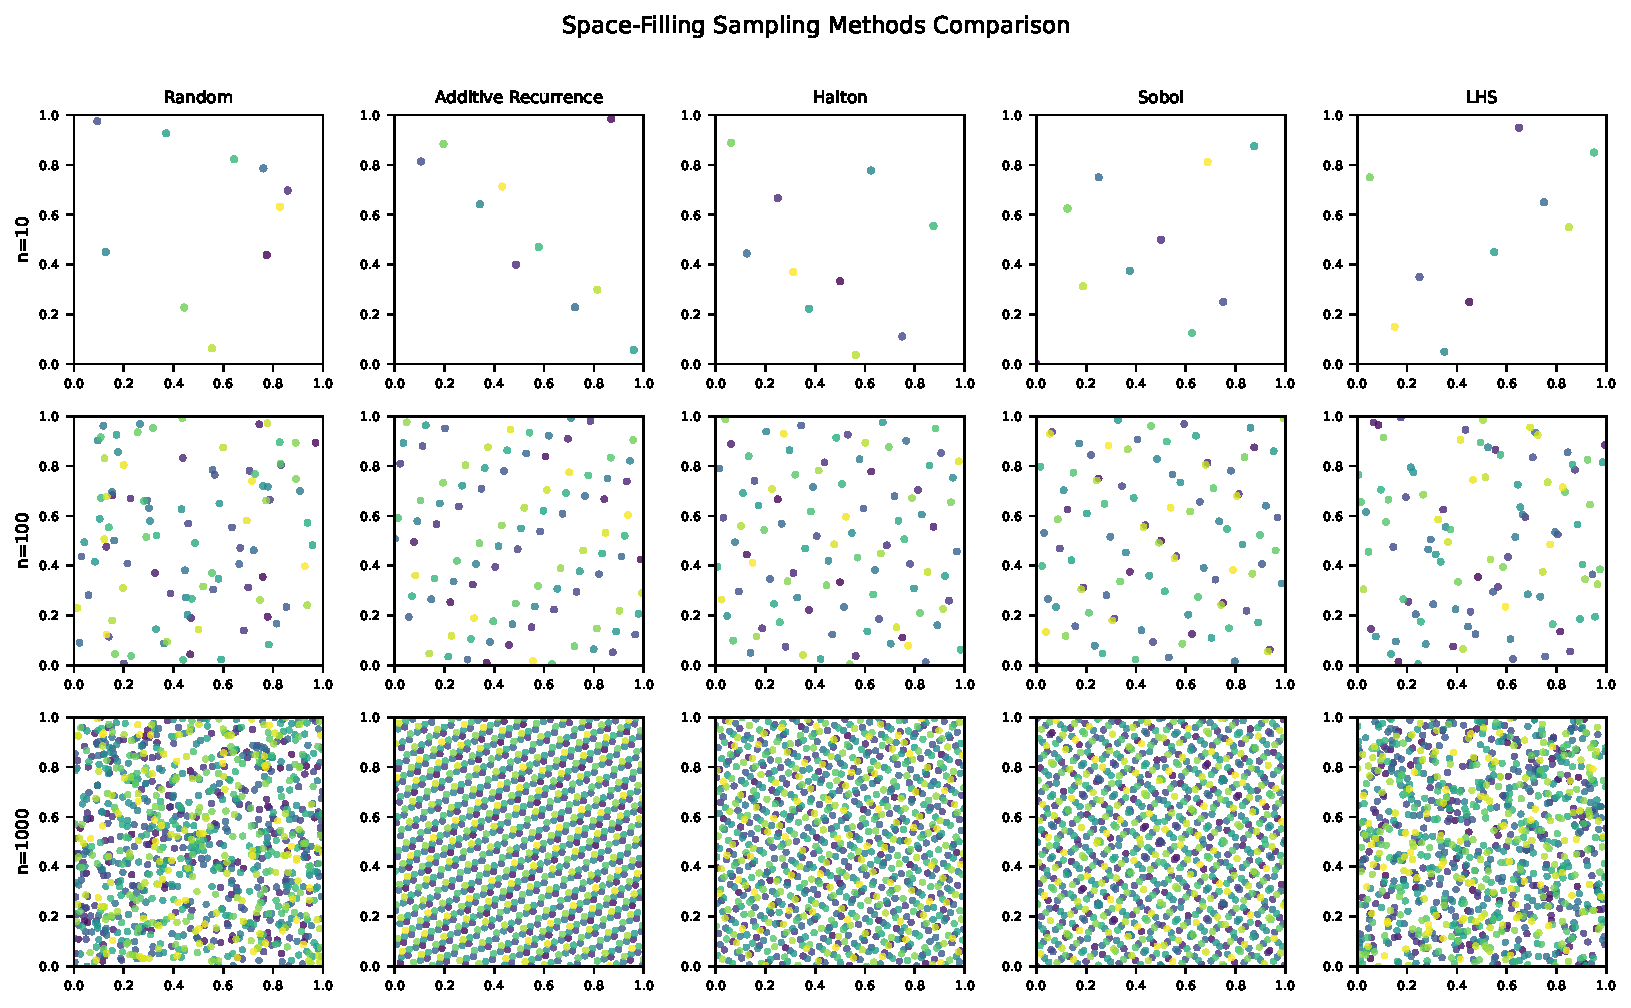
\includegraphics[width=\linewidth]{comparison_methods}
    \vspace{0.2em}
    \small Rows: $n = 10, 100, 1000$ points.
    Columns: Random, Additive Recurrence, Halton, Sobol, LHS (Uniform Projection).
    Colors encode order of sampling.

    \column{0.41\textwidth}
    \begin{block}{Observations}
      \begin{itemize}
        \item \textbf{Random}: clusters and gaps
        \item \textbf{Additive Recurrence}: diagonal banding
        \item \textbf{Halton}: excellent 2D coverage, may show patterns in high-$n$
        \item \textbf{Sobol}: very uniform, best for moderate $n$
        \item \textbf{LHS}: one-per-stratum guarantee, but no inter-dimensional structure
      \end{itemize}
    \end{block}
    \begin{alertblock}{Rule of Thumb}
      For $n \le 10$ dims: Sobol / Halton.\\
      For any $n$: optimized LHS (Morris-Mitchell).\\
      For subsets: greedy or exchange selection.
    \end{alertblock}
  \end{columns}
\end{frame}

% =============================================================================
\section{Summary \& Exercises}
% =============================================================================

\begin{frame}[allowframebreaks]{Summary}
  \begin{block}{Chapter 16 Key Concepts}
    \begin{enumerate}
      \item \textbf{Full Factorial}: evaluates all combinations on a grid.
            $\mathcal{O}(m^n)$ samples --- only practical for small $n$.
      \item \textbf{Random Sampling}: draws $m$ independent uniform samples.
            Simple but prone to clustering.
      \item \textbf{Uniform Projection Plans (LHS)}: one point per stratum in
            each dimension. Better 1D marginals; $\mathcal{O}(m)$ samples.
      \item \textbf{Stratified Sampling}: generalization that ensures
            sub-region coverage; LHS is a special case.
      \item \textbf{Discrepancy}: measures deviation of empirical distribution
            from uniform over all axis-aligned rectangles $H$.
      \item \textbf{Fill Distance}: largest radius uncovered ball in $\mathcal{X}$.
      \item \textbf{Morris-Mitchell Criterion} $\Phi_q$: minimizes
            $(\sum d_i^{-q})^{1/q}$; encourages large minimum pairwise distance.
    \end{enumerate}
  \end{block}

  \framebreak

  \begin{block}{Key Algorithms}
    \begin{tabular}{lll}
      \toprule
      Algorithm & Method & Use Case \\
      \midrule
      16.1 & Full factorial grid & Small $n$ (grid search) \\
      16.2 & Uniform projection plan & LHS generation \\
      16.3 & Pairwise distances & Plan evaluation \\
      16.4 & Compare plans & Ranking plans \\
      16.5 & Mutation & LHS optimization \\
      16.6 & Morris-Mitchell $\Phi_q$ & Quality metric \\
      16.7 & Max-fill distance & Subset metric \\
      16.8 & Greedy subset & Space-filling subset \\
      16.9 & Exchange subset & Improved subset \\
      16.10 & Additive recurrence & Quasi-random \\
      16.11 & Halton & Quasi-random \\
      \bottomrule
    \end{tabular}
  \end{block}

  \framebreak

  \begin{columns}
    \column{0.5\textwidth}
    \begin{block}{Monte Carlo Integration Rate}
      \begin{tabular}{ll}
        \toprule
        Method & Error rate \\
        \midrule
        Random (MC) & $\mathcal{O}(m^{-1/2})$ \\
        Quasi-random (QMC) & $\mathcal{O}((\log m)^n / m)$ \\
        \bottomrule
      \end{tabular}
      \vspace{0.3em}

      For large $m$ and small $n$, QMC is much faster to converge.
    \end{block}

    \column{0.46\textwidth}
    \begin{block}{Python Libraries}
      \begin{itemize}
        \item \texttt{scipy.stats.qmc}: Sobol, Halton, LHS
        \item \texttt{numpy.random}: pseudo-random
        \item \texttt{pyDOE2}: Latin Hypercube (extended)
        \item \texttt{SALib}: sensitivity analysis designs
      \end{itemize}
    \end{block}
  \end{columns}
\end{frame}

\begin{frame}[allowframebreaks]{16.9 Selected Exercises}
  \begin{exampleblock}{Exercise 16.1 --- Curse of Dimensionality}
    An $n$-dimensional hypercube of side $\ell$ filling half the volume
    of the unit hypercube satisfies $\ell^n = 1/2$, so:
    \[
      \ell = 2^{-1/n} \xrightarrow{n\to\infty} 1
    \]
    For $n=2$: $\ell = 1/\sqrt{2} \approx 0.707$.
    For $n=10$: $\ell = 2^{-0.1} \approx 0.933$.
    The side length approaches 1, meaning we need to search
    almost the entire space to cover half its volume!
  \end{exampleblock}

  \begin{exampleblock}{Exercise 16.2 --- Concentration of Measure}
    For a random point $\mathbf{x}$ uniform in the $n$-ball:
    \[
      P(\|\mathbf{x}\|_2 > 1-\epsilon)
        = 1 - P(\|\mathbf{x}\|_2 \le 1-\epsilon)
        = 1 - (1-\epsilon)^n \to 1
    \]
    As $n\to\infty$, \emph{all} mass concentrates near the surface.
    Random sampling becomes increasingly inefficient in high dimensions.
  \end{exampleblock}

  \framebreak

  \begin{exampleblock}{Exercise 16.3 --- Morris-Mitchell \& Translation Invariance}
    Sampling plan $X = \{[\cos(2\pi i/10),\,\sin(2\pi i/10)]\}_{i=1}^{10}$.
    Adding $[2,3]$ to every point: $\Phi_2(X)$ \textbf{does not change}.

    \textit{Reason}: $\Phi_q$ depends only on \emph{pairwise distances},
    and translation shifts all points equally, leaving all pairwise distances
    $\|\mathbf{x}^{(i)} - \mathbf{x}^{(j)}\|$ unchanged.
  \end{exampleblock}

  \begin{exampleblock}{Exercise 16.4 --- Why $c$ Must Be Irrational}
    If $c = a/b$ (rational), the additive recurrence:
    \[
      x^{(k)} = x^{(0)} + k\frac{a}{b} \pmod{1}
    \]
    After $b$ steps: $x^{(k+b)} = x^{(0)} + (k+b)\frac{a}{b} \pmod{1}
      = x^{(k)} + a \pmod{1} = x^{(k)}$.
    The sequence is \emph{periodic} with period $b$ and only covers
    $b$ distinct points, not a dense filling of $[0,1]$.
  \end{exampleblock}
\end{frame}

% --- FINAL SLIDE -------------------------------------------------------------
\begin{frame}{Chapter 16 --- Take-Home Messages}
  \begin{columns}
    \column{0.52\textwidth}
    \begin{block}{Key Principles}
      \begin{itemize}
        \item Function evaluations are expensive: choose sample points wisely
        \item Full factorial is impractical for $n > 4$
        \item Latin Hypercube (UPP) gives good 1D coverage with only $m$ points
        \item Quasi-random sequences (Halton, Sobol) beat random for integration
        \item Optimize LHS with Morris-Mitchell criterion $\Phi_q$
        \item For subset selection: greedy or exchange algorithms
      \end{itemize}
    \end{block}

    \column{0.44\textwidth}
    \begin{alertblock}{Design Space Coverage}
      As dimension $n$ grows:
      \begin{itemize}
        \item Volume concentrates in corners
        \item All points near the surface of high-dim balls
        \item More samples needed to cover the same fraction
        \item No sampling plan fully solves the curse of dimensionality
      \end{itemize}
    \end{alertblock}
    \vspace{0.4em}
    \begin{center}
      \large\textit{``Covering the space of designs\\
        is the first step toward finding\\
        the best design.''}
    \end{center}
  \end{columns}
\end{frame}

\end{document}
